\section{Discussion Of Test Results 讨论试验结果}

\begin{sidewaystable*}[!p]
    \centering
    \caption{Results of aging tests on Skabo clay}
    \addtocounter{table}{-1}
    \vspace{-12pt}
    \renewcommand{\tablename}{表}
    \caption{Skabo黏土的时效试验结果}
    \vspace{-8pt}
    \renewcommand{\tablename}{Table}
    \tabcolsep=0.8mm
    \begin{tabularx}{\textwidth}{lllXXllllllllllllll}
        \toprule
        \multirowcell{2}[-20pt][l]{Depth:\\m} & \multirow{2}*[-25pt]{Type} & \multirowcell{2}[-20pt][l]{Time of\\consolidation} & \multicolumn{2}{l}{\makecell[l]{Consolidation\\pressure: $\rm{kg/cm^2}$}} &  &  & \multicolumn{6}{l}{$(\sigma_1-\sigma_3)_{\max}$} & \multicolumn{6}{l}{$(\sigma_1'/\sigma_3')_{\max}$} \\\cmidrule(lr){4-5}\cmidrule(lr){8-13}\cmidrule(lr){14-19}
         & & & $\sigma_1$ & $\sigma_3$ & $w_i:\%$ & $w_f:\%$ & $\varepsilon_f:\%$ & \makecell[l]{($\sigma_1-\sigma_3$):\\$\rm{kg/cm^2}$} & \makecell[l]{$\Delta{u}$:\\$\rm{kg/cm^2}$} & $A$ & $\sigma_1'/\sigma_3'$ & \makecell[l]{Time to\\failure: min} & $\varepsilon:\%$ & \makecell[l]{($\sigma_1-\sigma_3$):\\$\rm{kg/cm^2}$} & \makecell[l]{$\Delta{u}$:\\$\rm{kg/cm^2}$} & $A$ & $\sigma_1'\sigma_3'$ & \makecell[l]{Time to\\failure: min}\\
        \midrule
        15.10  & CIU   & 3 days & 2.5   & 2.5   & 41.6  & 33.1  & 3.8   & 1.75  & 1.63  & 0.93  & 3.02  & 200   & 8.3   & 1.74  & 1.81  & 1.04  & 3.53  & 404 \\     15.45  & CIU   & 4 days & 2.5   & 2.5   & 48.2  & 38.2  & 3.3   & 1.70  & 1.59  & 0.94  & 2.87  & 223   & 8.4   & 1.67  & 1.82  & 1.09  & 3.45  & 448 \\     15.75  & CAU   & 5 days & 2.5   & 1.5   & 39.4  & 34.4  & 1.9   & 1.76  & 0.59  & 0.78  & 2.94  & 335   & 9.4   & 1.66  & 0.77  & 1.16  & 3.28  & 1128 \\     15.85  & CAU   & 6 days & 2.5   & 1.5   & 40.0  & 33.4  & 2.3   & 1.78  & 0.72  & 0.93  & 3.28  & 307   & 10.6  & 1.68  & 0.90  & 1.33  & 3.79  & 1255 \\     15.40  & CIU   & 2 weeks & 2.5   & 2.5   & 40.6  & 32.7  & 3.6   & 1.89  & 1.57  & 0.83  & 3.04  & 195   & 11.8  & 1.90  & 1.77  & 0.93  & 3.60  & 571 \\     15.50  & CIU   & 3 weeks & 2.5   & 2.5   & 41.2  & 32.4  & 4.3   & 1.90  & 1.63  & 0.86  & 3.18  & 230   & 9.3   & 1.85  & 1.72  & 0.93  & 3.37  & 456 \\     15.75  & CAU   & 4 weeks & 2.5   & 1.5   & 42.8  & 33.4  & 0.9   & 1.90  & 0.47  & 0.52  & 2.85  & 135   & 5.0   & 1.76  & 0.77  & 1.01  & 3.41  & 635 \\     15.85  & CAU   & 5 weeks & 2.5   & 1.5   & 43.2  & 33.5  & 0.8   & 1.78  & 0.48  & 0.62  & 2.74  & 124   & 11.8  & 1.46  & 1.00  & 2.17  & 3.93  & 1382 \\     15.35  & CIU   & 4 months & 2.5   & 2.5   & 47.8  & 37.6  & 2.0   & 1.85  & 1.31  & 0.71  & 2.55  & 116   & 10.1  & 1.65  & 1.80  & 1.09  & 3.36  & 452 \\     15.55  & CIU   & 5 months & 2.5   & 2.5   & 46.5  & 36.4  & 2.2   & 1.97  & 1.40  & 0.71  & 2.78  & 135   & 8.9   & 1.77  & 1.79  & 1.02  & 3.49  & 435 \\     16.10  & CAU   & 6 months & 2.5   & 1.5   & 41.9  & 35.4  & 0.5   & 1.74  & 0.36  & 0.49  & 2.53  & 99    & 12.0  & 1.32  & 0.91  & 2.84  & 3.24  & 1481 \\     16.20  & CAU   & 7 months & 2.5   & 1.5   & 43.5  & 36.2  & 0.5   & 2.02  & 0.34  & 0.34  & 2.74  & 100   & 11.0  & 1.54  & 0.92  & 1.70  & 3.66  & 1270 \\ 
        \bottomrule
    \end{tabularx}%
    \label{table:2}%
    \vspace{10pt}
    \caption{Results of aging tests on Skabo clay}
    \addtocounter{table}{-1}
    \vspace{-12pt}
    \renewcommand{\tablename}{表}
    \caption{Skabo黏土的时效试验结果}
    \vspace{-8pt}
    \renewcommand{\tablename}{Table}
    \begin{tabularx}{\textwidth}{llXXXXXXXXXXXXl}
        \toprule
        \multirowcell{2}[-6pt][l]{Type of\\test:} & \multirowcell{2}[-6pt][l]{Time of \\consolidation} & \multicolumn{2}{l}{Water content:} & \multicolumn{6}{l}{At $(\sigma_1-\sigma_3)_{\max}$} & \multicolumn{5}{l}{At $(\sigma_1'/\sigma_3')_{\max}$} \\\cmidrule(lr){3-4}\cmidrule(lr){5-10}\cmidrule(lr){11-15}
         & & $w_i$ & $w_f$ & $\varepsilon:\%$ & $\frac{(\sigma_1-\sigma_3)/2}{p}$ & $\sigma_1'/\sigma_3'$ & $\phi'$ & $D_M:\%$ & $A_f$ & $\varepsilon:\%$ & $\sigma_1'/\sigma_3'$ & $\phi'_u$ & $A$ & $\frac{\Delta{u}}{p}+1-K$ \\
         \midrule
         CIU & \makecell[l]{3 days\\2 weeks\\4 months} & \makecell[l]{44.9\\40.9\\37.0} & \makecell[l]{35.7\\32.5\\37.0} & \makecell[l]{3.6\\4.0\\2.1} & \makecell[l]{0.346\\0.379\\0.382} & \makecell[l]{2.95\\3.12\\2.67} & \makecell[l]{29.6°\\31.0°\\27.0°} & \makecell[l]{85\\90\\78} & \makecell[l]{0.94\\0.85\\0.71} & \makecell[l]{~8.4\\10.6\\~9.5} & \makecell[l]{3.49\\3.49\\3.43} & \makecell[l]{33.7°\\33.7°\\33.2°} & \makecell[l]{1.07\\0.93\\1.05} & \makecell[l]{0.72\\0.70\\0.72}\\
         CAU & \makecell[l]{3 days\\2 weeks\\4 months} & \makecell[l]{39.7\\43.0\\42.7} & \makecell[l]{33.9\\33.4\\35.8} & \makecell[l]{2.1\\0.9\\0.5} & \makecell[l]{0.354\\0.368\\0.376} & \makecell[l]{3.11\\2.80\\2.64} & \makecell[l]{30.8°\\28.3°\\26.8°} & \makecell[l]{88\\85\\77} & \makecell[l]{0.88\\0.57\\0.42} & \makecell[l]{10.0\\~8.4\\11.5} & \makecell[l]{3.54\\3.67\\3.45} & \makecell[l]{34.0°\\33.9°\\33.4} & \makecell[l]{1.24\\1.59\\2.27} & \makecell[l]{0.73\\0.75\\0.77} \\
        \bottomrule
    \end{tabularx}
    \label{table:3}
\end{sidewaystable*}


\begin{paracol}{2}
    
    Since all tests were performed in duplicate and because samples consolidated isotropically as well as anisotropically were allowed to age for three different periods, the test series includes in total twelve tests. The details of the test results are collected in \autoref{table:2} and some of the most important characteristics are summarized in \autoref{table:3}.

    \switchcolumn

    由于所有试验均一式两份进行,并且由于各向同性和各向异性固结的样品可以老化三个不同的时期,因此试验系列总共包括十二个试验。 \cntableref{table:2}收集了试验结果的详细信息,\cntableref{table:3}总结了一些最重要的特性。

    \switchcolumn*

    In \autoref{table:2} the failure parameters are listed, whereby it has been distinguished between the bulk failure of the sample at the peak value of the principal stress difference $(\sigma_1-\sigma_3)_{\max}$ and the ultimate failure of the soil skeleton occurring at maximum effective principal stress ratio $(\sigma_1'/\sigma_3')_{\max}$.

    \switchcolumn
       
    在\cntableref{table:2}中列出了破坏参数,从而区分了在主应力差$(\sigma_1-\sigma_3)_{\max}$峰值处的样品整体破坏和在最大有效主应力比$(\sigma_1'/\sigma_3')_{\max}$下发生的土体骨架的最终破坏。
    
    \switchcolumn*

    Before discussing the effect of the age on the shear strength characteristics, it is of importance to realize that there was no appreciable reduction in water content of the samples during the aging periods. This observation is confirmed by the measurements of the final water contents, see \autoref{table:3}, which do not show any regular decrease with the period of aging.

    \switchcolumn

    在讨论时效对剪切强度特性的影响之前,重要的是要认识到,时效期间样品的含水量没有明显降低。 最终水含量的测量结果证实了这一观察结果,请参见\cntableref{table:3},\cntableref{table:3}没有显示出随时间的任何规律性下降。

    \switchcolumn*

    From the shear-strength characteristics computed at the peak values of $(\sigma_1-\sigma_3)$ and $\sigma_1'/\sigma_3'$ and listed in \autoref{table:2} and \autoref{table:3} the following conclusions can be drawn: 

    \switchcolumn
       
    根据在$(\sigma_1-\sigma_3)$和$\sigma_1'/\sigma_3'$的峰值处计算并在\cntableref{table:2}和\cntableref{table:3}中列出的抗剪强度特性,可以得出以下结论:
     
    \switchcolumn*
    
    \noindent \emph{At $(\sigma_1-\sigma_3)_{\max}$ the effect of an increase of period of aging is:}
    
    ($a$) the undrained shear strengt $\dfrac{1}{2}(\sigma_1-\sigma_3)/p$ increase slightly; 

    ($b$) the pore-pressure parameter $A_f$ decreases; 

    ($c$) the strain at failure decreases; 

    ($d$) the angle of shearing resistance$\phi'$ mobilized at $(\sigma_1-\sigma_3)_{\max}$ decreases and the degree of mobilization defined as: $D_M=\tan\phi'/\tan\phi'_u$ thus decreases.

    \noindent \emph{At $(\sigma_1'-\sigma_3')_{\max}$ the effect is:}

    ($e$) the maximum principal effective stress ratio $\sigma_1'-\sigma_3'$ remains unchanged and so does the ultimate angle of shearing resistance $\phi'_u$;

    ($f$) the pore-pressure parameter A remains unchanged for the samples consolidated isotropically, but increases for the anisotropically consolidated samples.

    \switchcolumn

    \noindent \emph{在$(\sigma_1-\sigma_3)_{\max}$处,时间增加的影响为:}

    ($a$) 不排水的剪切强度$\dfrac{1}{2}(\sigma_1-\sigma_3)/p$略有增加;  

    ($b$) 孔隙压力参数$A_f$减小;  

    ($c$) 破坏应变降低;

    ($d$) 在$(\sigma_1-\sigma_3)_{\max}$处调动的抗剪角$\phi'$减小,将调动程度定义为:$D_M=\tan\phi'/\tan\phi'_u$,因此也相应减小。

    \noindent \emph{在$(\sigma_1'-\sigma_3')_{\max}$处,影响为为:}

   ($e$) 最大主有效应力比$\sigma_1'-\sigma_3'$保持不变,抗剪极限角$\phi'_u$也保持不变;

   ($f$) 对于各向同性固结的样品,孔隙压力参数$A$保持不变,但对于各向异性固结的样品,参数$A$则增加。

   \switchcolumn*

   The conclusions drawn may well be useful for an evaluation of the effect of time on the conventionally used shear strength parameters, but they contribute only little to a fundamental understanding of the change of properties of a clay occurring when it is left at a sustained consolidation pressure for a period of time. Much can however be learned from a study of the stress-strain properties and for this purpose the test results have been plotted in \autoref{figure:2} and \autoref{figure:3}. For a comparison of the stress-strain properties of a number of tests it has previously been found convenient to make use of the following equation which is generally valid and holds good for any strain :

   \switchcolumn

   得出的结论可能对评估时间对常规使用的剪切强度参数的影响很有用,但对于基本了解黏土保持一段时间持续固结压力时所发生的特性变化的作用不大。然而,从应力-应变特性的研究中可以学到很多,为此目的,试验结果绘制在\cnfigureref{figure:2}和\cnfigureref{figure:3}中。为了比较许多试验的应力-应变特性,以前发现很方便利用以下等式,该等式通常有效,并且对任何应变都适用: 

\end{paracol}

\begin{align}
    \frac{\sigma_1-\sigma_3}{p}=(\sigma_1'/\sigma_3'-1)\left[1-\left(\frac{\Delta{u}}{p}+(1-K)\right)\right]
\end{align}
\begin{figure*}
    \begin{minipage}[t]{0.51\textwidth}
        \centering
        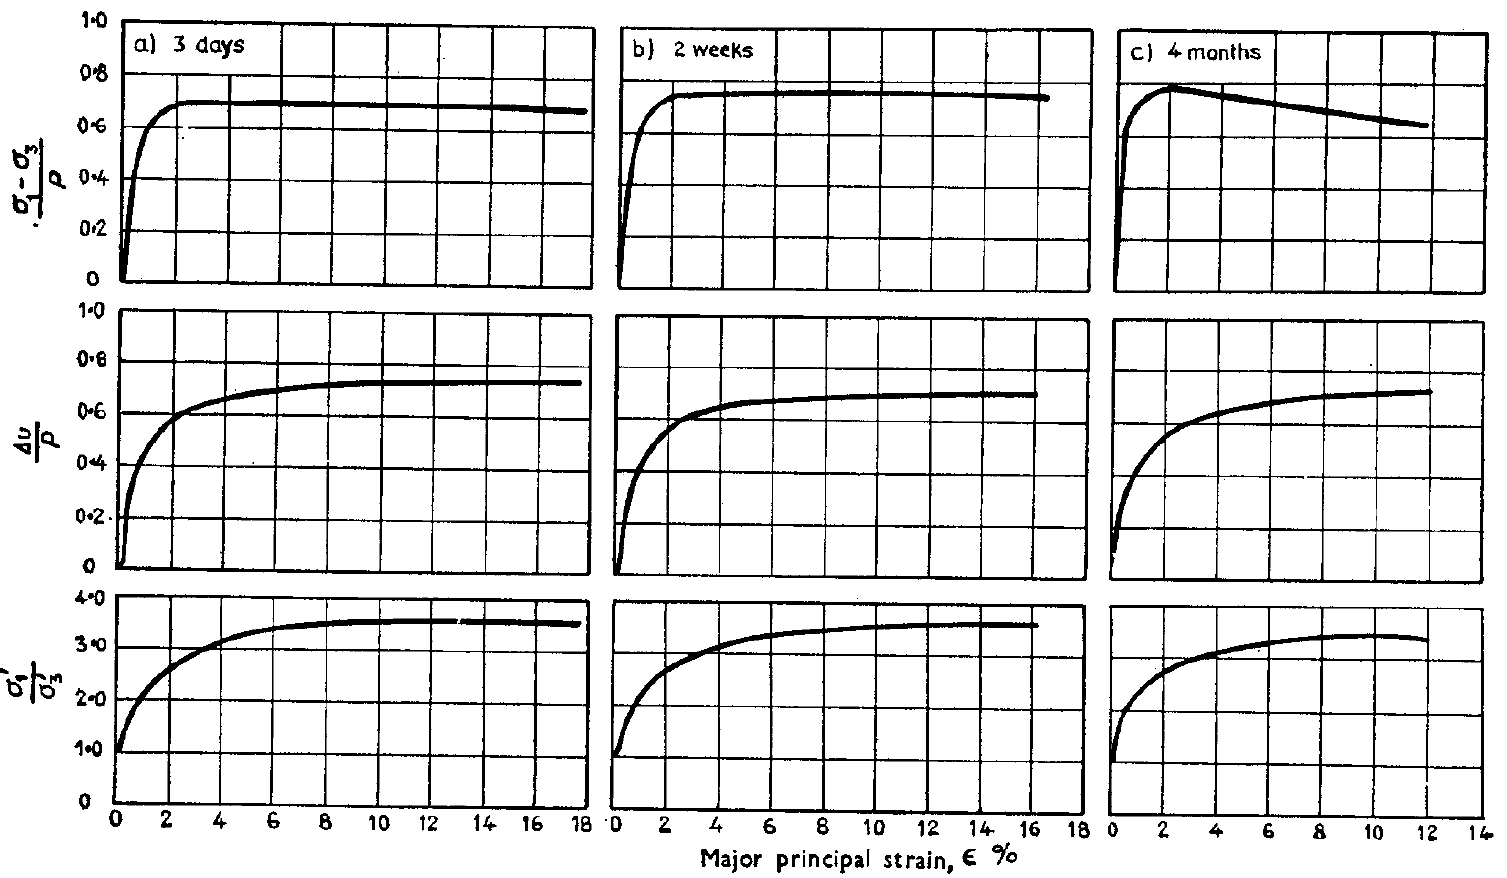
\includegraphics[width=\textwidth]{figures/figure-2.png}
        \caption{Results of consolidated undrained triaxial tests on samples consolidated isotropically for various periods of times: (a) 3 days, (b) 2 weeks, (c) 4 months. Consolidation pressure 25 $\rm{kg/sq\cdot{cm}}$. Each curve represents the average of two tests.}
        \addtocounter{figure}{-1}
        \vspace{-5pt}
        \renewcommand{\figurename}{图}
        \caption{各向同性固结样品在不同时间段的固结不排水三轴试验结果:(a)3天,(b)2周,(c)4个月。 固结压力25$\rm{kg/sq\cdot{cm}}$。 每条曲线代表两次试验的平均值。}
        \renewcommand{\figurename}{Figure}
        \label{figure:2}
    \end{minipage}
    \begin{minipage}[t]{0.44\textwidth}
        \centering
        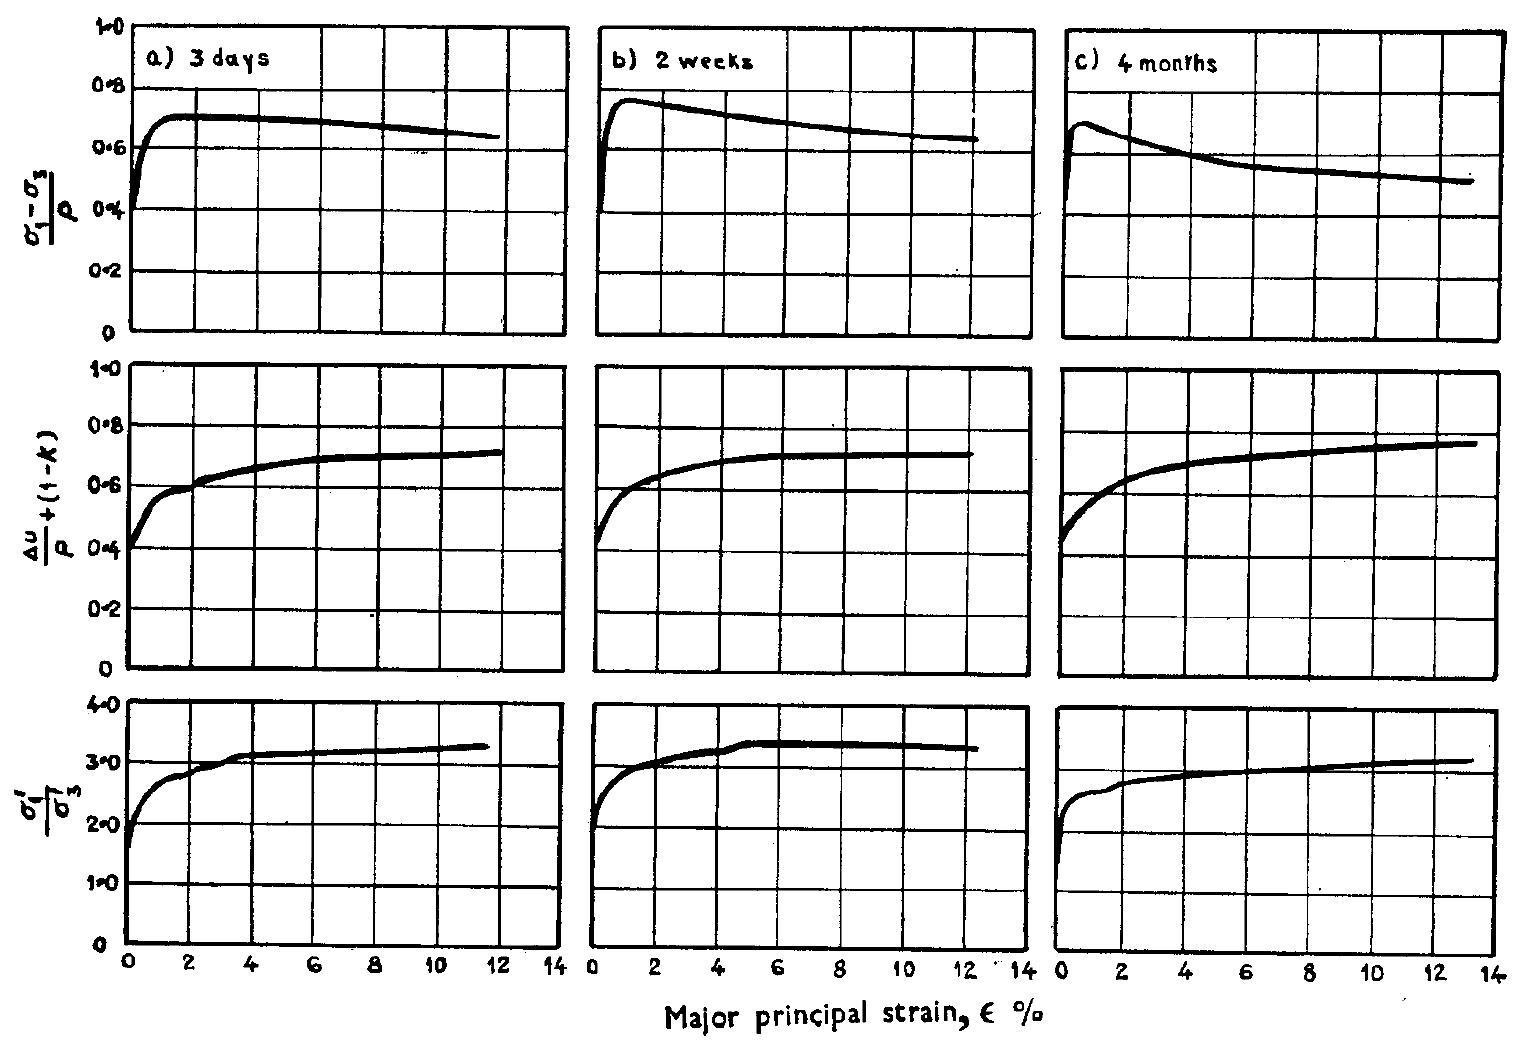
\includegraphics[width=\textwidth]{figures/figure-3.png}
        \caption{Results of consolidated undrained triaxial tests on samples consolidated anisotropically for various periods of times: (a) 3 days, (b) 2 weeks, (c) 4 months.
        Consolidation pressure $p_1=2.5\rm{kg/sq\cdot{cm}},p_2=p_3=1.5\rm{kg/sq\cdot{cm}}$. Each curve represents the average of two tests}
        \addtocounter{figure}{-1}
        \vspace{-5pt}
        \renewcommand{\figurename}{图}
        \caption{在不同时间段进行各向异性固结的样品的固结不排水三轴试验结果:(a)3天,(b)2周,(c)4个月。固结压力$p_1=2.5\rm{kg/sq\cdot{cm}},p_2=p_3=1.5\rm{kg/sq\cdot{cm}}$。每条曲线代表两次试验的平均值}
        \renewcommand{\figurename}{Figure}
        \label{figure:3}
    \end{minipage}
\end{figure*}

\begin{paracol}{2}
    
    \noindent in which $p$ and $Kp$ represent the major and minor principal consolidation pressures. In this equation $\sigma_1'/\sigma_3'-1$ and $\Delta{u}/p$ are considered to be independent functions of the strain and these functions will be discussed separately.

    \switchcolumn

    \noindent 式中$p$和$Kp$代表主要和次要固结应力。在该方程中,$\sigma_1'/\sigma_3'-1$和$\Delta{u}/p$被认为是应变的独立函数,并且将分别讨论这些函数。

\end{paracol}